%% LaTeX-Beamer template for KIT design
%% by Erik Burger, Christian Hammer
%% title picture by Klaus Krogmann
%%
%% version 2.4
%%
%% mostly compatible to KIT corporate design v2.0
%% http://intranet.kit.edu/gestaltungsrichtlinien.php
%%
%% Problems, bugs and comments to
%% burger@kit.edu

%% Class options
%%   aspect ratio options: 
%%   -- 16:9 (default)
%%   -- 4:3
%%   language options: 
%%   -- en (default)
%%   -- de
%%   position of navigation bar:
%%   -- navbarinline (default): bottom of the white canvas
%%   -- navbarinfooter : more compressed variant inside the footer
%%   -- navbarside : side bar at the left of the white canvas
%%   -- navbaroff : none
%% example: \documentclass[16:9,de,navbarside]{sdqbeamer}

\documentclass[16:9,en,navbarside]{sdqbeamer} 
 
%% TITLE PICTURE

% if a custom picture is to be used on the title page, copy it into the 'logos'
% directory, in the line below, replace 'myimage' with the 
% filename (without extension) and uncomment the following line
% (picture proportions: 63 : 20 for standard, 169 : 40 for wide
% *.eps format if you use latex+dvips+ps2pdf, 
% *.jpg/*.png/*.pdf if you use pdflatex)

\titleimage{customtitle}

%% GROUP LOGO 

% for a custom group logo, copy your file into the 'logos'
% directory, insert the filename in the line below and uncomment it

% \grouplogo{mylogo}

% (*.eps format if you use latex+dvips+ps2pdf,
% *.jpg/*.png/*.pdf if you use pdflatex)

%% GROUP NAME

% for groups other than SDQ, please insert in the line below and uncomment it
% \groupname{My group}

% the presentation starts here 

\title[Investigation of Ontologies in Software-Engineering-(Meta-)Research]{Proseminar work: \\ Investigation of Ontologies in Software-Engineering-(Meta-)Research}
\subtitle{Advisor: Dipl.-Inform. Angelika Kaplan}
\author{Dmitrii Seletkov}

% Bibliography 

\usepackage[citestyle=authoryear,bibstyle=numeric,hyperref,backend=biber]{biblatex}
\usepackage{multicol}
\addbibresource{presentation.bib}
\bibhang1em

\begin{document}

%title page
\KITtitleframe

%table of contents
\begin{frame}{Outline}
%\begin{multicols}{2}
\tableofcontents
%\end{multicols}
\end{frame}

\section{Motivation}
\begin{frame}{Motivation}
\begin{itemize}
\item Retrieving and transferring Knowledge: essential part of human being
\pause
\item \textbf{But}: the most amount of Knowledge is understandable only for humans
\pause
\item Ontologies make Knowledge understandable for computers as well, that provides:
    \begin{itemize}
        \item Supporting humans in Knowledge transferring process
        \item Opportunity to analyze and generate new knowledge automatically by machines
    \end{itemize}
\pause
\item Useful for Software Engineering
    \begin{itemize}
        \item Encapsulate the results of thousands Software Engineering experiments
        \item Make possible to analyze them and find out the best Software Engineering practice
    \end{itemize} 
\end{itemize}
\end{frame}

\section{Foundations}
\subsection{Ontologies in Computer Science}
\begin{frame}{Ontology in Computer Science}
\pause
\begin{alertblock}{Def. Ontology in Computer Science}
    \begin{itemize}
        \item \enquote{an explicit specification of a conceptualization} [\cite{Gru93}]
        \item Conceptualization: abstract model of some knowledge domain
        \item Explicit specification: classes, concepts, terms
    \end{itemize}
\end{alertblock}
\end{frame}

\begin{frame}{Ontology languages}
    
    \begin{exampleblock}{Well-known examples}
        \begin{itemize}
            \item ER-Diagrams and UML-Diagrams
            \item Good for understanding and representing of Knowledge, but still made for humans
        \end{itemize}
    \end{exampleblock}
    \pause
    \begin{block}{Description Logic (DL)}
        \begin{itemize}
            \item Family of knowledge representation languages  
            \pause
            \item Has formal semantics and instruments of logical analysis
            \pause
            \item Has different dialects and implementations such as OWL
            \pause
            \item OWL: Ontology Web Language, current standard and XML-based
            \pause
        \end{itemize}
    \end{block}
   
\end{frame}


\begin{frame}{Description Logic}
    \begin{alertblock}{The main feature:  \textbf{separation} between \textbf{Terminology} and \textbf{Assertions}}

    
    \begin{figure}
		\centering
		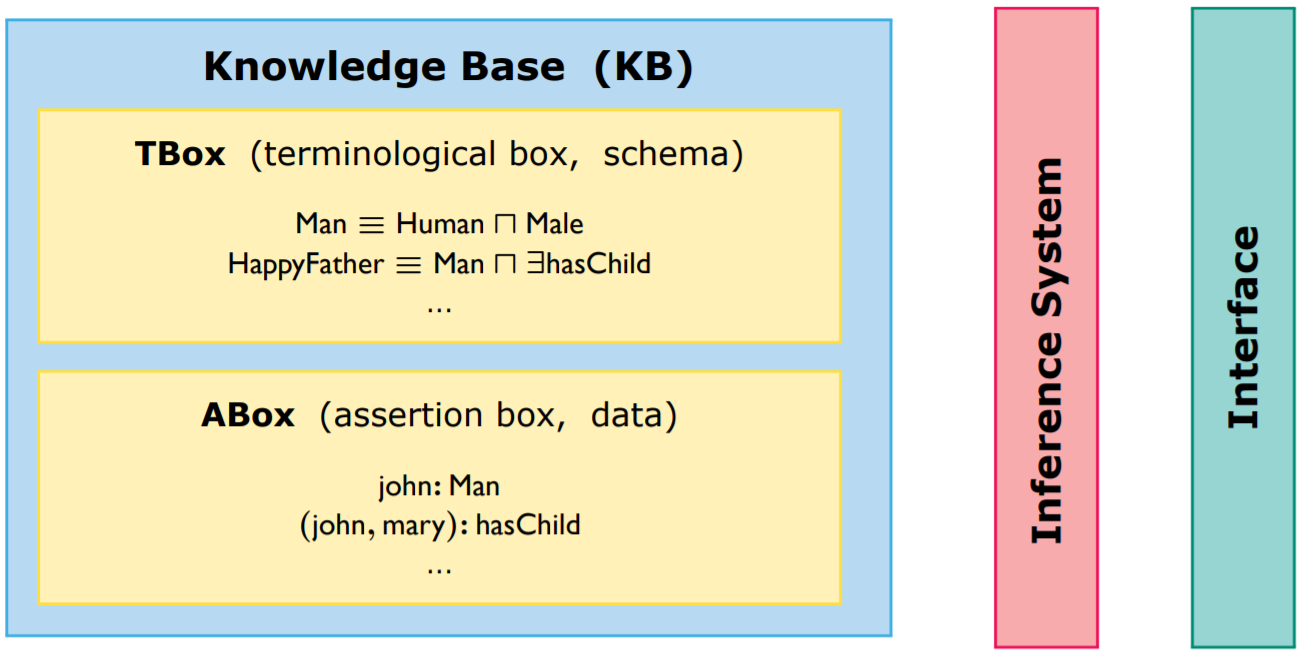
\includegraphics[width=8cm]{images/ELDL.PNG}
		\caption{Architecture of DL [\cite{Kon10}]}
		\label{fig:ArchDL}
	\end{figure}

	\end{alertblock}
\end{frame}


\subsection{Meta-Research}
\begin{frame}{Meta-research (1)}
\pause
     \begin{block}{Motivation}
        \begin{itemize}
			\item Research practices suffer from lack of systematization and inefficiency
			\pause
			\item Problems with data sharing, replications of experiments and their ownership
			\pause
			\item Urgent need of the science for the evaluation of diverse researches to improve the existing research practices and create the new ones
		\end{itemize}
    \end{block}
    \pause
    \begin{alertblock}{Def. Meta-Research}
       The use of scientific methodology to study science itself 
    \end{alertblock}
\end{frame}

\begin{frame}{Meta-Research (2)}
     \begin{block}{Areas of Meta-Research [\cite{Ioa15}]}
        \begin{enumerate}
            \setbeamercovered{transparent}
			\item<1->{\textbf{Methods}:} practices for performing research  (\textbf{e.g.} study design, methods, statistics). 
			\item<2->{\textbf{Reporting}:} publications of standards and study registrations  (\textbf{e.g.} study registration, information to patients, public and policy-makers)
			
			\item<3->\textbf{{Reproducibility}:} methods for verifying research (\textbf{e.g.} sharing data and methods, replicability)
			
			\item<4->{\textbf{Evaluation}:} approvements for scientific quality (\textbf{e.g.} pre- and post-publication peer reviews, research funding criteria).
			 
			\item<5->{\textbf{Incentives}:} rewards and penalties for research (\textbf{e.g.} promotion criteria, penalties in research evaluation).
		\end{enumerate}
    \end{block}
\end{frame}

\section{Ontologies in Software-Engineering-Meta-Research}

\begin{frame}{Ontologies in Software-Engineering-Meta-Research}
\pause
    \begin{figure}
		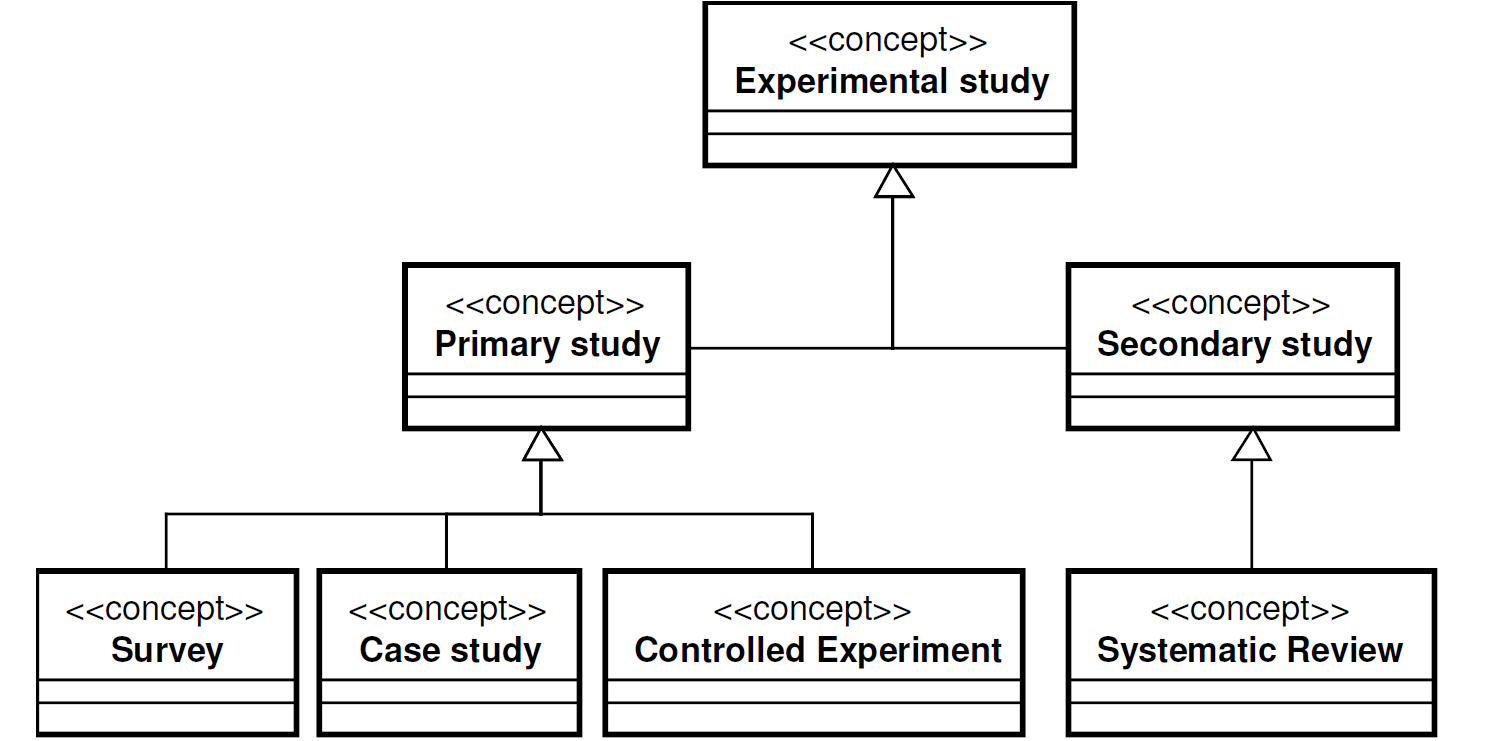
\includegraphics[width=9cm]{images/ClassificationStudies.PNG}
		\caption{Classification of empirical studies [\cite{Gar08}]}
	\end{figure}
\end{frame}


\subsection{Ontologies for Controlled Experiments on SE}
\begin{frame}{Ontology for Controlled Experiments on SE}
\begin{alertblock}{Problem}
    \begin{itemize}
        \item Sharing of knowledge among research groups
        \pause
        \item Requires \textbf{replication of Controlled Experiments} using Lab Packages
        \pause
        \item Lab Packages suffer from lack of standardization 
    \end{itemize}
\end{alertblock}
\pause
\begin{block}{Objectives}
\begin{itemize}
			\item Present an Ontology for experimental studies for knowledge transfer, assisting in designing, conducting and evaluating controlled experiments.
			\pause
			\item Validate the ontology, whilst instantiating it to a controlled experiment.
		\end{itemize}
\end{block}
\end{frame}

\begin{frame}{Ontology for Controlled Experiments on SE}
     \begin{figure}
		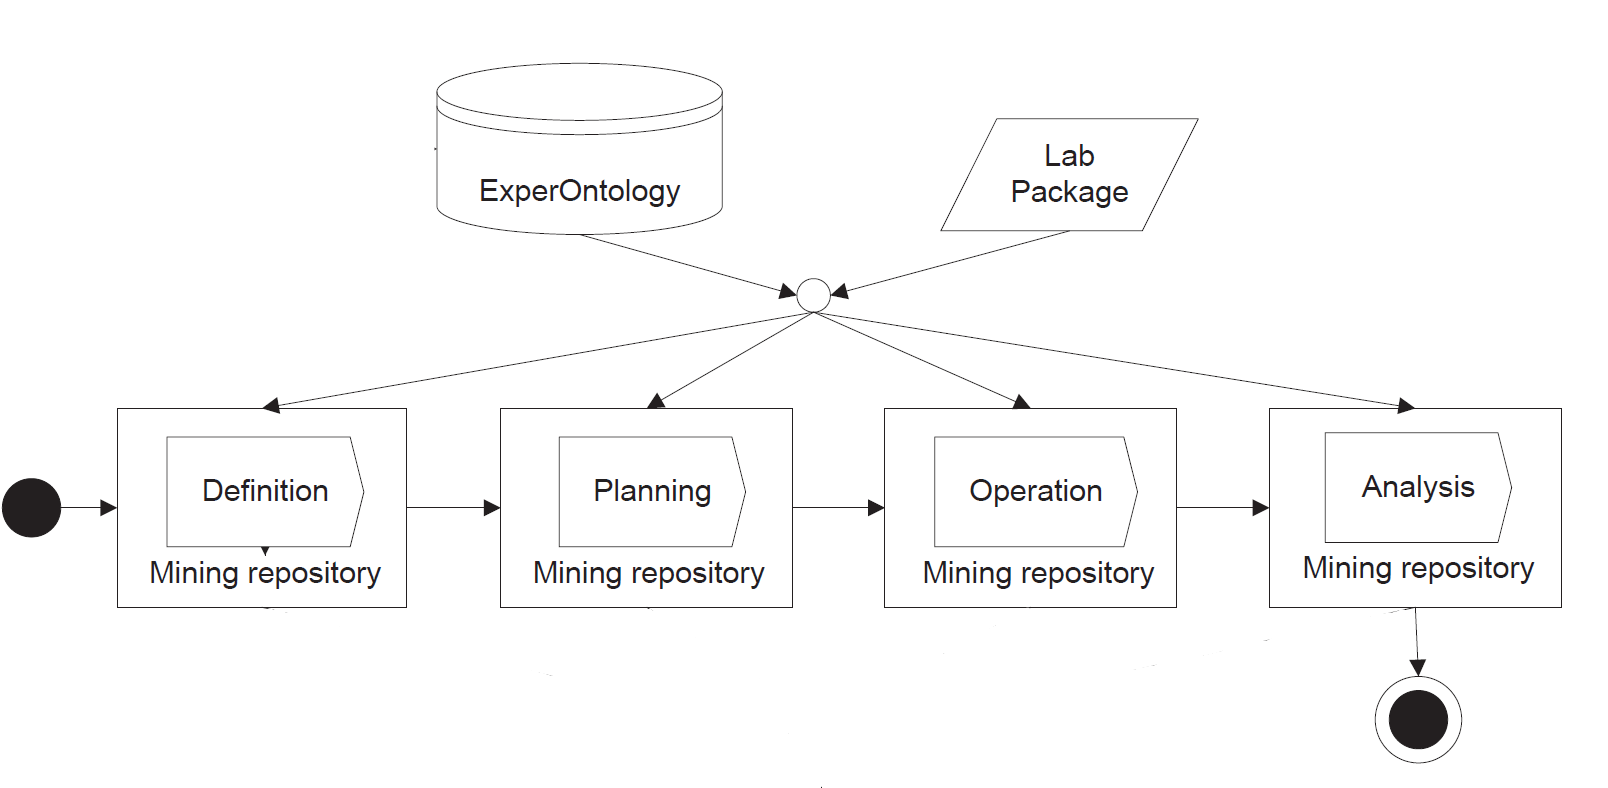
\includegraphics[width=9cm]{images/ExperOntology.png}
		\caption{Controlled Experiments phases [\cite{Gar11}]}
		\label{fig:ontforce}
	\end{figure}
\end{frame}

\begin{frame}{Ontology for Controlled Experiments on SE}
\begin{block}{Suggested Ontology (main concepts)}
\begin{multicols}{2}
\begin{enumerate}
        \setbeamercovered{transparent}
		\item<1> \textit{Lab Package} from \textit{Original Experiment} is used for \textit{Replication} and generation of a new \textit{Lab Package}.
		\item<2>  \textit{Experimenter Profile}: negative - lack of experience, positive - high experience
		\item<3> \textit{Original Experiment} and \textit{Replication} evaluated regarding to \textit{Validity}	
\end{enumerate}
\begin{figure}
		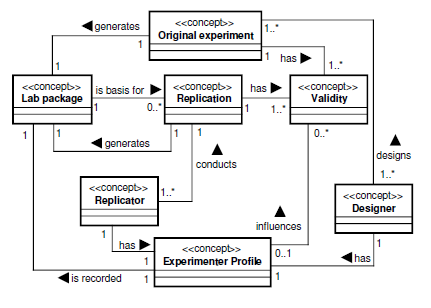
\includegraphics[width=5.5cm]{images/OntforCE.PNG}
		\caption{Ontology for Controlled Experiments [\cite{Gar08}]}
		\label{fig:ontforce}
	\end{figure}
\end{multicols}
\end{block}
\end{frame}

\begin{frame}{Ontology for Controlled Experiments on SE}
\begin{block}{Evaluation}
    \begin{itemize}
        \item Experiments [\cite{Bas87}] encapsulated in Lab Package 
        \item Comparing 3 testing techniques 
        \item 32 Subjects in \textbf{3 groups} with \textbf{3 testing techniques} for \textbf{3 types software}
    \end{itemize}
\end{block}
\pause
\begin{block}{Results}
    \begin{itemize}
        \item After instanciation of experiment into the ontology observe the missing values on the predicate
        \pause
        \item After look into experiment: indeed
        \pause
        \item Ontology: mechanism to improve the obtained data set from the Lab Package
    \end{itemize}
\end{block}
\end{frame}


\subsection{Ontology to support systematic reviews in SE}
\begin{frame}{Ontology to support systematic reviews in SE}
\pause
\begin{block}{Evidence-based Software Engineering [\cite{Kit04}]}
\begin{itemize}
   	\item Originates from Evidence-based Medicine
   	\pause
   	\item Purpose: determine what SE practice works, when, where and which tools
and standards needed
    \pause
    \item The main instrument: Systematic Reviews (SRs)
\end{itemize}
\end{block}
\end{frame}

\begin{frame}{Ontology to support systematic reviews in SE}
\begin{alertblock}{Problem}
\begin{itemize}
    \item Major challenge to strengthen the foundations of SE: \\produce knowledge that can be based on scientific methodology
\end{itemize}
\end{alertblock}
\pause
\begin{block}{Objectives}
    \begin{itemize}
		\item Present a template designed to support systematic reviews in SE
		\pause
		\item Introduce development of ontologies to describe knowledge regarding such experimental studies 
    \end{itemize}
\end{block}
\end{frame}

\begin{frame}{Ontology to support systematic reviews in SE}
\begin{exampleblock}{Systematic Review conduction process}
\begin{enumerate}
    \setbeamercovered{transparent}
    \item<1> \textbf{Planning}: research objectives and SR protocol
    \item<2> \textbf{Execution}: identify, select and evaluate primary studies
    \item<3> \textbf{Result Analysis}: extract and synthesize data from the the articles
    \begin{figure}
	    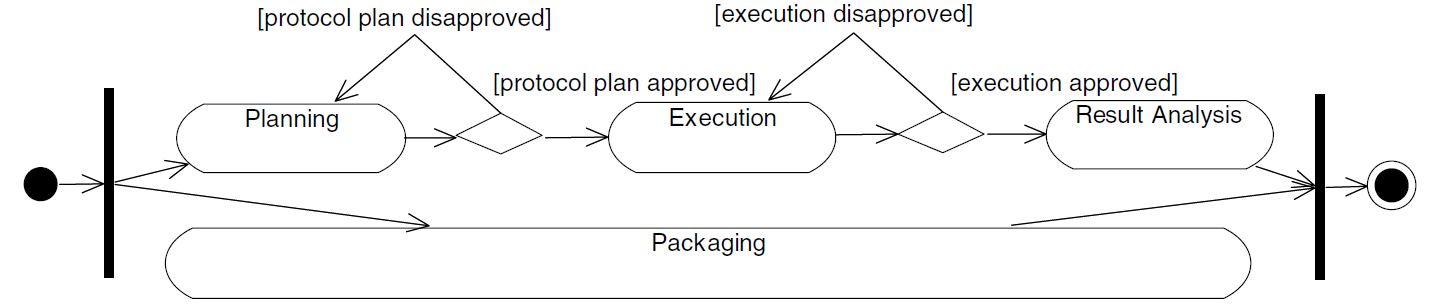
\includegraphics[width=11cm]{images/SRProcess.PNG}
	    \caption{Systematic Review conduction process [\cite{Bio07}]}
    \end{figure}
\end{enumerate}
\end{exampleblock}
\end{frame}

\begin{frame}{Systematic Review}
    \begin{figure}
		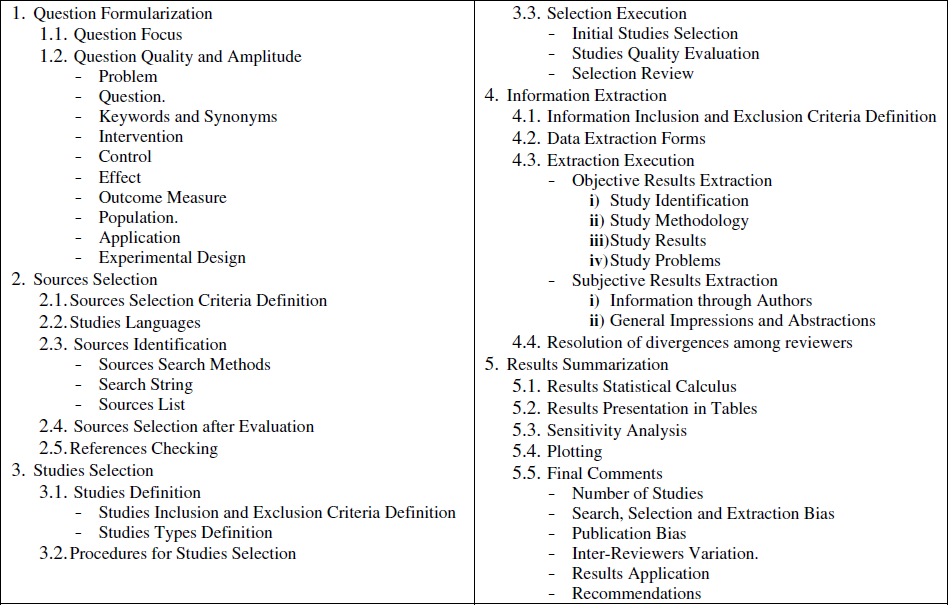
\includegraphics[width=9cm]{images/SRreviewprotocol.PNG}
		\caption{Systematic Review protocol template [\cite{Bio07}]}
	\end{figure}
\end{frame}

\begin{frame}{Systematic Review}
    \begin{figure}
		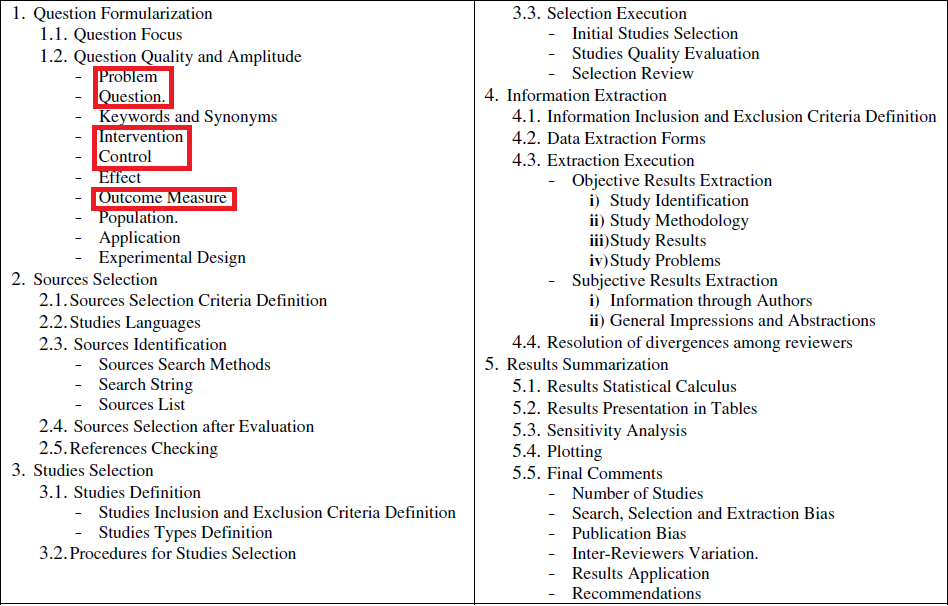
\includegraphics[width=9cm]{images/SRreviewprotocol2.PNG}
		\caption{Systematic Review protocol template [\cite{Bio07}]}
	\end{figure}
\end{frame}

\begin{frame}{Scientific Ontology}
\begin{block}{Suggested Ontology features}
    \begin{itemize}
        \setbeamercovered{transparent}
		\item<1-> Based on SR protocol template
		\item<2-> Level-structured
		\item<3-> Both taxonomic \textit{is\_a} and meronymic \textit{has} relations
		\item<4-> Level 0:  \textit{Experimental Method}, \textit{Primary Research} and \textit{Research Synthesis}
	    \item<5-> Next: only \textit{Primary Research}
	    \item<6-> But: similar for \textit{Experimental Method} and \textit{Research Synthesis}
	\end{itemize}
\end{block}
\end{frame}

\begin{frame}{Primary Research ontology}
    \begin{figure}
		
\includegraphics[width=12cm]{images/SROnt1.PNG}
	\end{figure}
\end{frame}

\begin{frame}{Primary Research ontology}
    \begin{figure}
		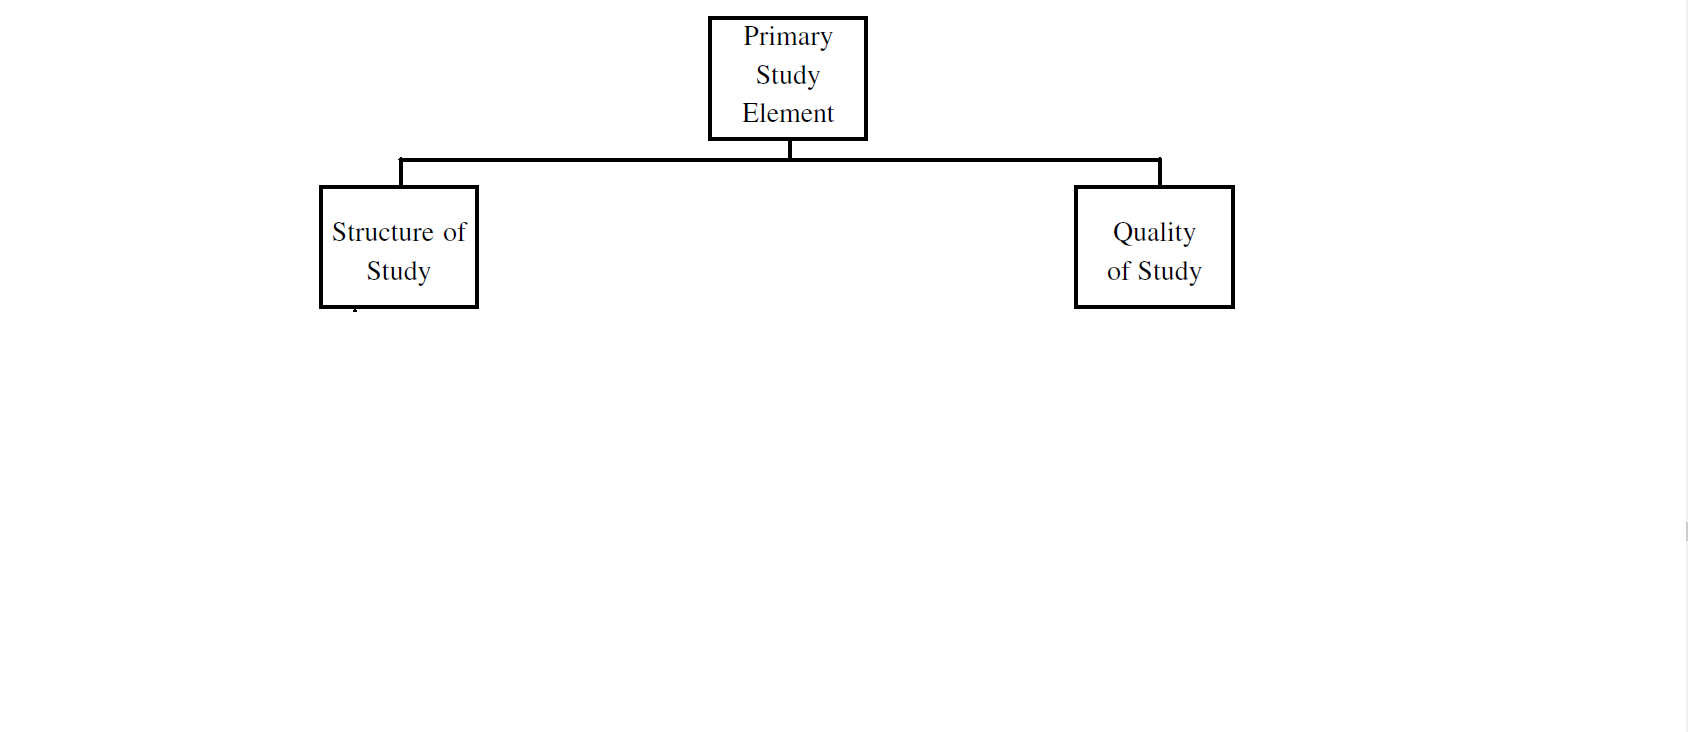
\includegraphics[width=12cm]{images/SROnt2.PNG}
	\end{figure}
\end{frame}

\begin{frame}{Primary Research ontology}
    \begin{figure}
		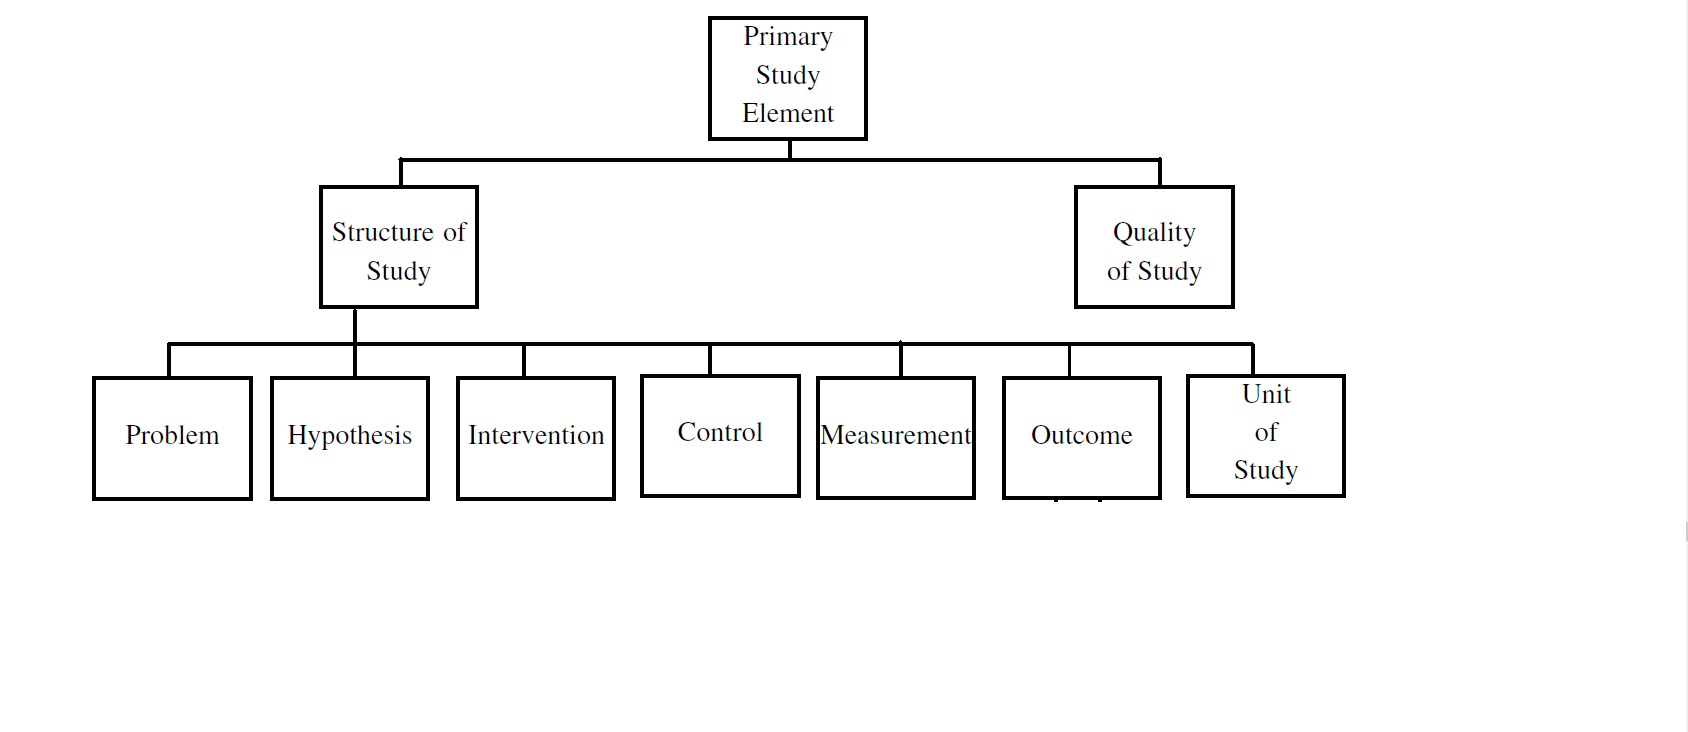
\includegraphics[width=12cm]{images/SROnt3.PNG}
	\end{figure}
\end{frame}

\begin{frame}{Primary Research ontology}
    \begin{figure}
		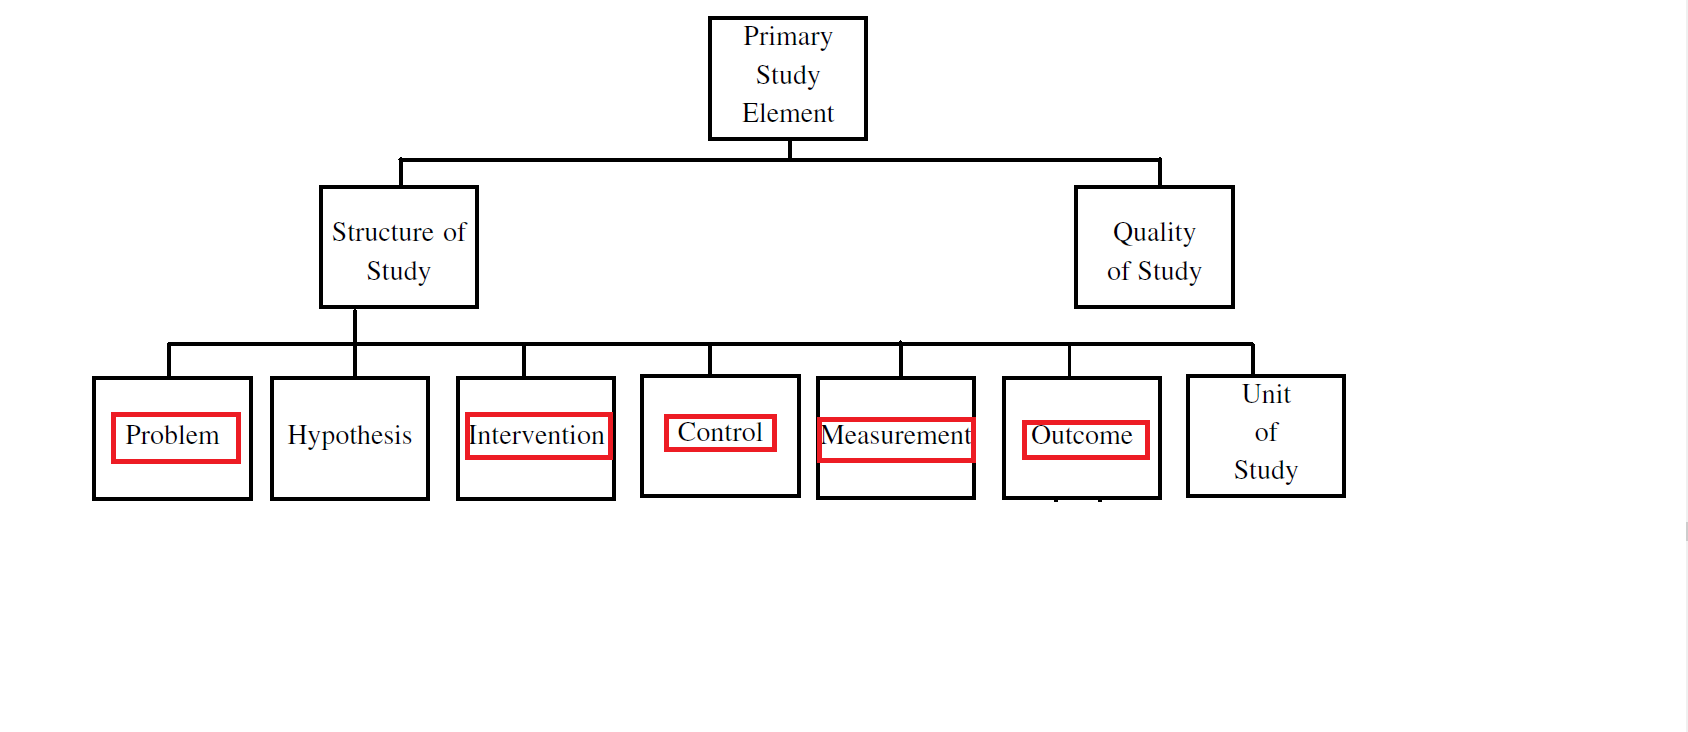
\includegraphics[width=12cm]{images/SROnt3.5.PNG}
	\end{figure}
\end{frame}

\begin{frame}{Primary Research ontology}
    \begin{figure}
		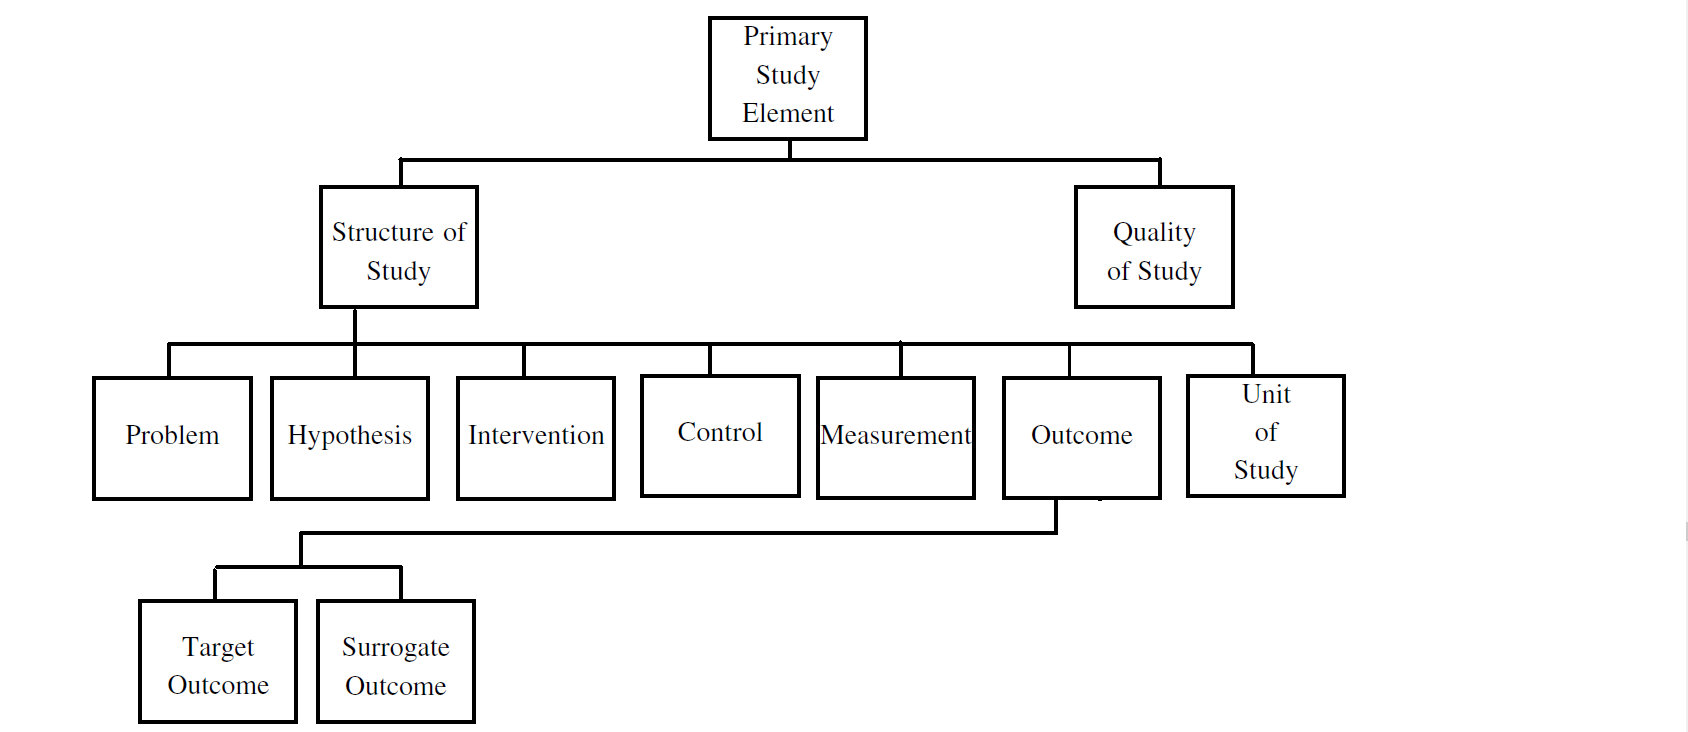
\includegraphics[width=12cm]{images/SROnt4.PNG}
	\end{figure}
\end{frame}

\begin{frame}{Primary Research ontology}
    \begin{figure}
		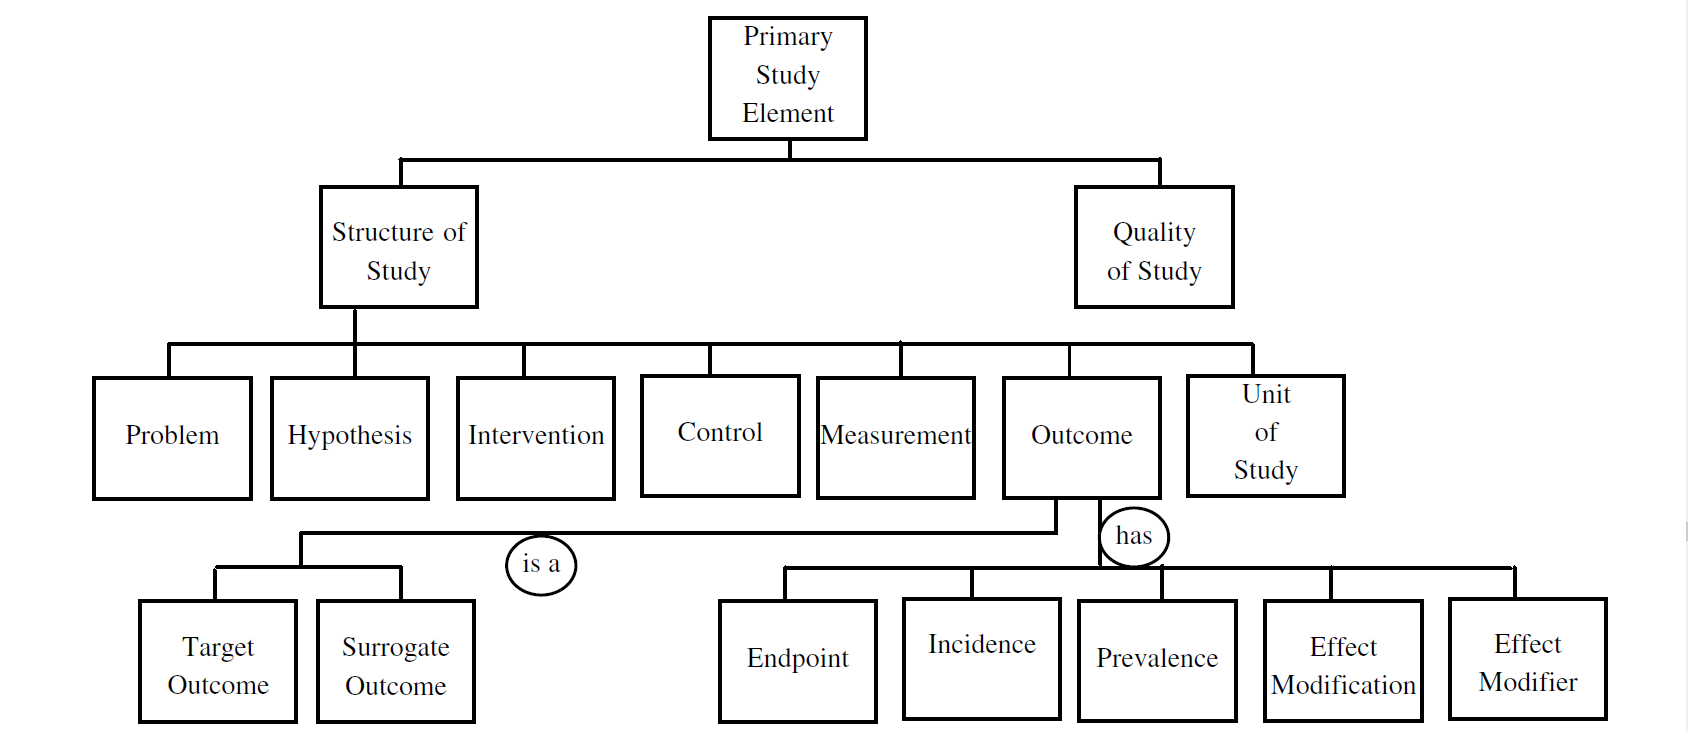
\includegraphics[width=12cm]{images/SROnt5.PNG}
		\caption{Primary Research ontology [\cite{Bio07}]}
	\end{figure}
\end{frame}

\begin{frame}{Ontology to support systematic reviews in SE}
\begin{block}{Result}  
    \begin{itemize}
        \item Observe: the ontology results in directly linked with Systematic review protocol template object.
        \pause
        \item Here only the small part. The full ontology conceptualizes on all roles in SR template
        \pause
        \item Powerful, comprehensive and covers all SR needs
    \end{itemize}
\end{block}
\end{frame}

\begin{frame}{Comparison}
\begin{block}{Similarities}
    \setbeamercovered{transparent}
    \begin{itemize}
        \item<1-> Adoption of ontologies: best for accumulate knowledge and formalize it
        \item<2-> Not a silver bullet: \textbf{but}, still enough for fulfilling a lot of objectives
        \item<3-> In Development: towards a comprehensive ontologies for all purposes
    \end{itemize}
\end{block}
\pause
\begin{block}{Differences}
\begin{itemize}
    \setbeamercovered{transparent}
    \item<4-> Ontology for supporting systematic reviews [\cite{Bio07}] belongs to Methods
    \item<5-> Ontology for Controlled Experiments [\cite{Gar08}] belongs to Reproducibility
    \item<6->  Used different ontology languages $\rightarrow$ barriers for applying them and making as standard 
    
\end{itemize}
\end{block}
\end{frame}


\section{Conclusion}
\begin{frame}{Conclusions}
\pause
\begin{block}{Ontologies}
    \setbeamercovered{transparent}
    \begin{itemize}
        \item<2-> The best tool for interchanging of pure information independent on languages, definitions and other syntactic barriers 
        \item<3-> Effectively reuse and standardize of the obtained knowledge
        \item<4-> Contemporary ontologies based on strictly defined in mathematical logic ontology languages 
    \end{itemize}
\end{block}
\pause
\begin{block}{Meta-Research}  
    \setbeamercovered{transparent}
    \begin{itemize}
		\item<5-> Research on research
		\item<6-> How researches should be conducted, what practices effective and in what fields
		\item<7-> Diversity of meta-research research: Methods, Reporting, Reproducibility, Evaluation, Incentives.
	\end{itemize}
\end{block}
\end{frame}
\begin{frame}{Conclusions}
\setbeamercovered{transparent}
\begin{block}{Ontologies in Software-Engineering-Meta-Research}
    \begin{itemize}
        \item<1-> Support determining the best SE practices using SRs in secondary studies 
        \item<2-> Useful for packaging of controlled experiments in primary studies
        \item<3-> Detection of inconsistencies in SE experiments
        \item<4-> No current standard
        \item<5-> Merging problem in future 
    \end{itemize}
\end{block}
\end{frame}

\appendix
\beginbackup

\begin{frame}[allowframebreaks]{References}
\printbibliography
\end{frame}

\backupend

\end{document}